\appendix
\chapter{Appendix}
This section includes the full implementation of the JSON printer, as well as 
the language for lesson plans, and additional information to provide further 
clarification on the report.

\newpage

\label{appendix_a}
\captionof{listing}{JSON Code of a Notebook Document
	\label{code:notebookmetada}}
	\begin{lstlisting}[language=json, 
	basicstyle=\linespread{1.1}\small\ttfamily] 
		{
			"cells": [
			{
				"cell_type": "markdown",
				"metadata": {},
				"source": []
			}
			],
			"metadata": {
				"kernelspec": {
					"display_name": "Python 3",
					"language": "python",
					"name": "python3"
				},
				"language_info": {
					"codemirror_mode": {
						"name": "ipython",
						"version": 3
					},
					"file_extension": ".py",
					"mimetype": "text/x-python",
					"name": "python",
					"nbconvert_exporter": "python",
					"pygments_lexer": "ipython3",
					"version": "3.9.1"
				}
			},
			"nbformat": 4,
			"nbformat_minor": 4
		}	
	\end{lstlisting}

\newpage

\captionof{listing}{Source Code for Language.Drasil.JSON.Print
\label{code:JSONPrint}}
\begin{lstlisting}[language=haskell1, 
	basicstyle=\linespread{1.1}\small\ttfamily]
	-- | Defines .json printers to generate Jupyter Notebooks
	
	-- | Generate a python notebook document (using json).
	-- build : build the SRS document in JSON format
	-- build': build the Jupyter Notbooks (lesson plans)
	genJSON :: PrintingInformation -> DocType -> L.Document -> Doc
	genJSON sm Jupyter doc = build (makeDocument sm doc)
	genJSON sm _       doc = build' (makeDocument sm doc)
		
	-- | Build the JSON Document, called by genJSON
	build :: Document -> Doc
	build (Document t a c) = 
		markdownB $$
		nbformat (text "# " <> pSpec t) $$
		nbformat (text "## " <> pSpec a) $$
		markdownE $$
		print' c $$
		markdownB' $$
		markdownE' $$
		makeMetadata $$
		text "}" 

	build' :: Document -> Doc
	build' (Document t a c) = 
		markdownB $$
		nbformat (text "# " <> pSpec t) $$
		nbformat (text "## " <> pSpec a) $$
		markdownE $$
		markdownB' $$ 
		print c $$
		markdownE' $$
		makeMetadata $$
		text "}" 

	-- | Helper for rendering a D from Latex print
	printMath :: D -> Doc
	printMath = (`runPrint` Math)
		
	-- | Helper for rendering LayoutObjects into JSON
	-- printLO is used for generating SRS
	printLO :: LayoutObj -> Doc
	printLO (Header n contents l) = nbformat empty $$ nbformat 
		(h (n + 1) <> pSpec contents) $$ refID (pSpec l)
	printLO (Cell layoutObs) = markdownCell $ vcat (map printLO layoutObs)
	printLO (HDiv _ layoutObs _) = vcat (map printLO layoutObs)
	printLO (Paragraph contents) = nbformat empty $$ nbformat 
		(stripnewLine (show(pSpec contents)))
	printLO (EqnBlock contents) = nbformat mathEqn
		where
			toMathHelper (PL g) = PL (\_ -> g Math)
			mjDelimDisp d  = text "$$" <> stripnewLine (show d) <> text "$$" 
			mathEqn = mjDelimDisp $ printMath $ toMathHelper $ TeX.spec contents
	printLO (Table _ rows r _ _) = nbformat empty $$ 
		makeTable rows (pSpec r)
	printLO (Definition dt ssPs l) = nbformat (text "<br>") $$ 
		makeDefn dt ssPs (pSpec l)
	printLO (List t) = nbformat empty $$ makeList t False
	printLO (Figure r c f wp) = makeFigure (pSpec r) (pSpec c) (text f) wp
	printLO (Bib bib) = makeBib bib
	printLO Graph{} = empty 
	printLO CodeBlock {} = empty
		
	-- printLO' is used for generating lesson plans
	printLO' :: LayoutObj -> Doc
	printLO' (HDiv ["equation"] layoutObs _) = markdownCell $ 
		vcat (map printLO' layoutObs)
	printLO' (Header n contents l) = markdownCell $ nbformat 
		(h (n + 1) <> pSpec contents) $$ refID (pSpec l)
	printLO' (Cell layoutObs) = vcat (map printLO' layoutObs)
	printLO' HDiv {} = empty
	printLO' (Paragraph contents) = markdownCell $ nbformat
		(stripnewLine (show(pSpec contents)))
	printLO' (EqnBlock contents) = nbformat mathEqn
		where
			toMathHelper (PL g) = PL (\_ -> g Math)
			mjDelimDisp d  = text "$$" <> stripnewLine (show d) <> text "$$" 
			mathEqn = mjDelimDisp $ printMath $ toMathHelper $ TeX.spec contents
	printLO' (Table _ rows r _ _) = markdownCell $ makeTable rows (pSpec r)
	printLO' Definition {} = empty
	printLO' (List t) = markdownCell $ makeList t False
	printLO' (Figure r c f wp) = markdownCell $ 
		makeFigure (pSpec r) (pSpec c) (text f) wp
	printLO' (Bib bib) = markdownCell $ makeBib bib
	printLO' Graph{} = empty 
	printLO' (CodeBlock contents) = codeCell $ codeformat $ cSpec contents
	
	-- | Called by build
	print :: [LayoutObj] -> Doc
	print = foldr (($$) . printLO) empty
	
	-- | Called by build'
	print' :: [LayoutObj] -> Doc
	print' = foldr (($$) . printLO') empty
	
	pSpec :: Spec -> Doc
	pSpec (E e) = text "$" <> pExpr e <> text "$"
	pSpec (a :+: b) = pSpec a <> pSpec b
	pSpec (S s) = either error (text . concatMap escapeChars) $ 
		L.checkValidStr s invalid
		where
			invalid = ['<', '>']
			escapeChars '&' = "\\&"
			escapeChars c = [c]
	pSpec (Sp s) = text $ unPH $ L.special s
	pSpec HARDNL = empty
	pSpec (Ref Internal r a) = reflink r $ pSpec a
	pSpec (Ref (Cite2 n) r a) = reflinkInfo r (pSpec a)(pSpec n)
	pSpec (Ref External r a) = reflinkURI r $ pSpec a
	pSpec EmptyS    = text ""
	pSpec (Quote q) = doubleQuotes $ pSpec q
	
	cSpec :: Spec -> Doc
	cSpec (E e)  = pExpr e 
	cSpec _      = empty
	
	-- | Renders expressions in JSON 
	-- (called by multiple functions)
	pExpr :: Expr -> Doc
	pExpr (Dbl d)        = text $ showEFloat Nothing d ""
	pExpr (Int i)        = text $ show i
	pExpr (Str s)        = doubleQuotes $ text s
	pExpr (Div n d)      = mkDiv "frac" (pExpr n) (pExpr d)
	pExpr (Row l)        = hcat $ map pExpr l
	pExpr (Ident s)      = text s
	pExpr (Label s)      = text s
	pExpr (Spec s)       = text $ unPH $ L.special s
	pExpr (Sub e)        = unders <> pExpr e
	pExpr (Sup e)        = hat <> pExpr e
	pExpr (Over Hat s)   = pExpr s <> text "&#770;"
	pExpr (MO o)         = text $ pOps o
	pExpr (Fenced l r e) = text (fence Open l) <> pExpr e <> 
		text (fence Close r)
	pExpr (Font Bold e)  = pExpr e
	pExpr e              = printMath $ toMath $ TeX.pExpr e
	
	-- | Renders operations in Markdown format
	pOps :: Ops -> String
	pOps IsIn     = "&thinsp;&isin;&thinsp;"
	pOps Integer  = "&#8484;"
	pOps Rational = "&#8474;"
	pOps Real     = "&#8477;"
	pOps Natural  = "&#8469;"
	pOps Boolean  = "&#120121;"
	pOps Comma    = ","
	pOps Prime    = "&prime;"
	pOps Log      = "log"
	pOps Ln       = "ln"
	pOps Sin      = "sin"
	pOps Cos      = "cos"
	pOps Tan      = "tan"
	pOps Sec      = "sec"
	pOps Csc      = "csc"
	pOps Cot      = "cot"
	pOps Arcsin   = "arcsin"
	pOps Arccos   = "arccos"
	pOps Arctan   = "arctan"
	pOps Not      = "&not;"
	pOps Dim      = "dim"
	pOps Exp      = "e"
	pOps Neg      = "-"
	pOps Cross    = "&#10799;"
	pOps VAdd     = " + "
	pOps VSub     = " - "
	pOps Dot      = "&sdot;"
	pOps Scale    = ""
	pOps Eq       = " = "
	pOps NEq      = "&ne;"
	pOps Lt       = "&thinsp;&lt;&thinsp;" 
	pOps Gt       = "&thinsp;&gt;&thinsp;"
	pOps LEq      = "&thinsp;&le;&thinsp;"
	pOps GEq      = "&thinsp;&ge;&thinsp;"
	pOps Impl     = " &rArr; "
	pOps Iff      = " &hArr; "
	pOps Subt     = " - "
	pOps And      = " &and; "
	pOps Or       = " &or; "
	pOps Add      = " + "
	pOps Mul      = ""
	pOps Summ     = "&sum"
	pOps Inte     = "&int;"
	pOps Prod     = "&prod;"
	pOps Point    = "."
	pOps Perc     = "%"
	pOps LArrow   = " &larr; "
	pOps RArrow   = " &rarr; "
	pOps ForAll   = " ForAll "
	pOps Partial  = "&part;"
	
	-- | Renders Markdown table, called by 'printLO'
	makeTable :: [[Spec]] -> Doc -> Doc
	makeTable [] _      = error "No table to print"
	makeTable (l:lls) r = refID r $$ nbformat empty $$ 
		(makeHeaderCols l $$ makeRows lls) $$ nbformat empty
	
	-- | Helper for creating table rows
	makeRows :: [[Spec]] -> Doc
	makeRows = foldr (($$) . makeColumns) empty
	
	-- | makeHeaderCols: Helper for creating table header row 
	-- (each of the column header cells)
	-- | makeColumns: Helper for creating table columns
	makeHeaderCols, makeColumns :: [Spec] -> Doc
	makeHeaderCols l = nbformat (text header) $$ 
		nbformat (text $ genMDtable ++ "|")
		where 
			header = show(text "|" <> hcat(punctuate (text "|") 
				(map pSpec l)) <> text "|")        
			c = count '|' header
			genMDtable = concat (replicate (c-1) "|:--- ")
	
	makeColumns ls = nbformat (text "|" <> hcat(punctuate 
		(text "|") (map pSpec ls)) <> text "|")
	
	count :: Char -> String -> Int
	count _ [] = 0
	count c (x:xs) 
		| c == x = 1 + count c xs
		| otherwise = count c xs
	
	-- | Renders definition tables (Data, General, Theory, etc.)
	makeDefn :: L.DType -> [(String,[LayoutObj])] -> Doc -> Doc
	makeDefn _ [] _  = error "L.Empty definition"
	makeDefn dt ps l = refID l $$ table [dtag dt] (tr (nbformat 
		(th (text "Refname")) $$ td	(nbformat(bold l))) $$ makeDRows ps)
		where dtag L.General  = "gdefn"
			    dtag L.Instance = "idefn"
			    dtag L.Theory   = "tdefn"
			    dtag L.Data     = "ddefn"
	
	-- | Helper for making the definition table rows
	makeDRows :: [(String,[LayoutObj])] -> Doc
	makeDRows [] = error "No fields to create defn table"
	makeDRows [(f,d)] = tr (nbformat (th (text f)) $$ td 
		(vcat $ map printLO d))
	makeDRows ((f,d):ps) = tr (nbformat (th (text f)) $$ td 
		(vcat $ map printLO d)) $$ makeDRows ps
	
	-- | Renders lists
	makeList :: ListType -> Bool -> Doc
	makeList (Simple items) _ = vcat $ map (\(b,e,l) -> mlref l 
		$ nbformat (pSpec b <> text ": " <> sItem e) $$ nbformat empty) items
	makeList (Desc items) bl = vcat $ map (\(b,e,l) -> pa $
		mlref l $ ba $ pSpec b <> text ": " <> pItem e bl) items
	makeList (Ordered items) bl = vcat $ map (\(i,l) -> mlref l 
		$ pItem i bl) items
	makeList (Unordered items) bl = vcat $ map (\(i,l) -> 
		mlref l $ pItem i bl) items
	makeList (Definitions items) _ = vcat $ map (\(b,e,l) -> nbformat $ li $ 
	mlref l $ pSpec b <> text " is the" <+> sItem e) items
	
	-- | Helper for setting up references
	mlref :: Maybe Label -> Doc -> Doc
	mlref = maybe id $ refwrap . pSpec
	
	-- | Helper for rendering list items
	pItem :: ItemType ->  Bool -> Doc
	pItem (Flat s) b = nbformat $ (if b then text " - " else 
		text "- ") <> pSpec s
	pItem (Nested s l) _ = vcat [nbformat $ text "- " <> 
		pSpec s, makeList l True]
		
	sItem :: ItemType -> Doc
	sItem (Flat s)     = pSpec s
	sItem (Nested s l) = vcat [pSpec s, makeList l False]
	
	-- | Renders figures in HTML
	makeFigure :: Doc -> Doc -> Doc -> L.MaxWidthPercent -> Doc
	makeFigure r c f wp = refID r $$ image f c wp
	
	-- | Renders assumptions, requirements, likely changes
	makeRefList :: Doc -> Doc -> Doc -> Doc
	makeRefList a l i = refID l $$ nbformat(i <> text ": " <> a)
	
	makeBib :: BibRef -> Doc
	makeBib = vcat .
		zipWith (curry (\(x,(y,z)) -> makeRefList z y x))
		[text $ sqbrac $ show x | x <- [1..] :: [Int]] . map renderCite
\end{lstlisting}

\newpage

\captionof{listing}{Source Code for Language.Drasil.JSON.Helpers
	\label{code:JSONHelpers}}
\begin{lstlisting}[language=haskell1, 
	basicstyle=\linespread{1.1}\small\ttfamily]
	-- | Defines helper functions for creating Jupyter Notebooks
		
	data Variation = Class | Id
	
	tr, td, figure, li, pa, ba :: Doc -> Doc
	-- | Table row tag wrapper
	tr     = wrap "tr" []
	-- | Table cell tag wrapper
	td     = wrap "td" []
	-- | Figure tag wrapper
	figure = wrap "figure" []
	-- | List tag wrapper
	li     = wrap' "li" []
	-- | Paragraph in list tag wrapper
	pa     = wrap "p" []
	-- | Bring attention to element wrapper.
	ba     = wrap "b" []
	
	ol, ul, table :: [String] -> Doc -> Doc
	-- | Ordered list tag wrapper
	ol     = wrap "ol"
	-- | Unordered list tag wrapper
	ul     = wrap "ul"
	-- | Table tag wrapper
	table  = wrap "table"
	
	nbformat :: Doc -> Doc
	nbformat s = text ("    " ++ J.encode (show s ++ "\n") ++ ",")
	
	codeformat :: Doc -> Doc
	codeformat s = text ("    " ++ J.encode (show s))
	
	wrap :: String -> [String] -> Doc -> Doc
	wrap a = wrapGen' vcat Class a empty
	
	wrap' :: String -> [String] -> Doc -> Doc
	wrap' a = wrapGen' hcat Class a empty
	
	wrapGen' :: ([Doc] -> Doc) -> Variation -> String -> Doc -> 
		[String] -> Doc -> Doc
	wrapGen' sepf _ s _ [] = \x -> 
		let tb c = text $ "<" ++ c ++ ">"
		in if s == "li" then sepf [tb s, x, tb $ '/':s] 
			else sepf [nbformat(tb s), x, nbformat(tb $ '/':s)]
	wrapGen' sepf Class s _ ts = \x ->
		let tb c = text $ "<" ++ c ++ " class=\\\"" ++ foldr1 (++) 
			(intersperse " " ts) ++ "\\\">"
		in let te c = text $ "</" ++ c ++ ">"
		in sepf [nbformat(tb s), x, nbformat(te s)]
	wrapGen' sepf Id s ti _ = \x ->
		let tb c = text ("<" ++ c ++ " id=\\\"") <> ti <> text "\\\">"
				te c = text $ "</" ++ c ++ ">"
		in  sepf [nbformat(tb s), x, nbformat(te s)] 
	
	refwrap :: Doc -> Doc -> Doc
	refwrap = flip (wrapGen' vcat Id "div") [""]
	
	refID :: Doc -> Doc 
	refID i = nbformat $ text "<a id=\"" <> i <> text "\"></a>"
	
	-- | Helper for setting up links to references
	reflink :: String -> Doc -> Doc
	reflink ref txt = text "[" <> txt <> text ("](#" ++ ref ++ ")")
	
	-- | Helper for setting up links to external URIs
	reflinkURI :: String -> Doc -> Doc
	reflinkURI ref txt = text ("<a href=\\\"" ++ ref ++ "\\\">") 
		<> txt <> text "</a>"
	
	-- | Helper for setting up figures
	image :: Doc -> Doc -> MaxWidthPercent -> Doc
	image f c 100 = 
		figure $ vcat [
		nbformat $ img [("src", f), ("alt", c)]]
	image f c wp =
		figure $ vcat [
		nbformat $ img [("src", f), ("alt", c), ("width", 
			text $ show wp ++ "%")]]
	
	h :: Int -> Doc
	h n | n < 1 = error "Illegal header (too small)"
			| n > 4 = error "Illegal header (too large)"          
			| otherwise = text (hash n)
				where hash 1 = "# "
							hash 2 = "## "
							hash 3 = "### "
							hash 4 = "#### "
							hash _ = "Illegal header"
	
	-- | Curly braces.
	br :: Doc -> Doc
	br x = text "{" <> x <> text"}"
	
	mkDiv :: String -> Doc -> Doc -> Doc
	mkDiv s a0 a1 = (H.bslash <> text s) <> br a0 <> br a1
	
	stripnewLine :: String -> Doc
	stripnewLine s = hcat (map text (splitOn "\n" s))
	
	-- | Helper for building Markdown cells
	markdownB, markdownB', markdownE, markdownE' :: Doc
	markdownB  = text "{\n \"cells\": [\n  {\n   \"cell_type\": 
		\"markdown\",\n   \"metadata\": {},\n   \"source\": [\n" 
	markdownB' = text "  {\n   \"cell_type\": \"markdown\",\n   
		\"metadata\": {},\n   \"source\": [\n" 
	markdownE  = text "    \"\\n\"\n   ]\n  },"
	markdownE' = text "    \"\\n\"\n   ]\n  }\n ],"
		
	-- | Helper for building code cells
	codeB, codeE :: Doc
	codeB = text "  {\n   \"cell_type\": \"code\",\n   
		\"execution_count\": null,\n   \"metadata\": {},\n   
		\"outputs\": [],\n   \"source\": [" 
	codeE  = text "\n   ]\n  },"
		
	-- | Helper for generate a Markdown cell
	markdownCell :: Doc -> Doc
	markdownCell c = markdownB' <> c <> markdownE
		
	-- | Helper for generate a code cell
	codeCell :: Doc -> Doc
	codeCell c = codeB <> c <> codeE
		
	-- | Generate the metadata necessary for a notebook document
	makeMetadata :: Doc  
	makeMetadata = vcat [
		text " \"metadata\": {", 
		vcat[
			text "  \"kernelspec\": {", 
			text "   \"display_name\": \"Python 3\",", 
			text "   \"language\": \"python\",",
			text "   \"name\": \"python3\"", 
			text "  },"],
		vcat[
			text "  \"language_info\": {", 
			text "   \"codemirror_mode\": {", 
			text "    \"name\": \"ipython\",",
			text "    \"version\": 3",
			text "   },"],
		text "   \"file_extension\": \".py\",", 
		text "   \"mimetype\": \"text/x-python\",",
		text "   \"name\": \"python\",",
		text "   \"nbconvert_exporter\": \"python\",",
		text "   \"pygments_lexer\": \"ipython3\",",
		text "   \"version\": \"3.9.1\"",
		text "  }",
		text " },",
		text " \"nbformat\": 4,", 
		text " \"nbformat_minor\": 4" 
	]
\end{lstlisting}

\newpage

\captionof{listing}{Source Code for DocLang.Notebook
	\label{code:docLang_notebook}}
\begin{lstlisting}[language=haskell1, 
	basicstyle=\linespread{1.1}\small\ttfamily]	
	-- * Section Constructors	
	-- | Section constructors for the Lesson Plans
	intro, learnObj, review, caseProb, summary, appendix, 
		reference, example :: [Contents] -> [Section] -> Section
	intro     cs ss = section (titleize  Docum.introduction) 
		cs ss introLabel
	learnObj  cs ss = section (titleize' Docum.learnObj)    
		cs ss learnObjLabel
	review    cs ss = section (titleize  Docum.review)      
		cs ss reviewLabel
	caseProb  cs ss = section (titleize  Docum.caseProb)     
		cs ss caseProbLabel
	example   cs ss = section (titleize  Docum.example)      
		cs ss exampleLabel
	summary   cs ss = section (titleize  Docum.summary)      
		cs ss summaryLabel
	appendix  cs ss = section (titleize  Docum.appendix)     
		cs ss appendixLabel
	reference cs ss = section (titleize' Docum.reference)   
		cs ss referenceLabel
	
	--Labels--
	sectionReferences :: [Reference]
	sectionReferences = [introLabel, learnObjLabel, 
		docPurposeLabel, referenceLabel, reviewLabel, 
		appendixLabel, summaryLabel, exampleLabel]
	
	-- * Section References
	
	-- | Individual section reference labels. 
	-- Used in creating example sections for the notebook.
	introLabel, learnObjLabel, docPurposeLabel, referenceLabel, 
		reviewLabel, caseProbLabel, appendixLabel, summaryLabel, 
		exampleLabel :: Reference
	introLabel      = makeSecRef "Intro"            
		$ titleize  Docum.introduction
	learnObjLabel   = makeSecRef "LearnObj"         
		$ titleize' Docum.learnObj
	docPurposeLabel = makeSecRef "DocPurpose"       
		$ titleize  Docum.prpsOfDoc
	referenceLabel  = makeSecRef "References"       
		$ titleize'	Docum.reference
	reviewLabel     = makeSecRef "Review"           
		$ titleize  Docum.review
	caseProbLabel   = makeSecRef "CaseProb"         
		$ titleize  Docum.caseProb
	appendixLabel  = makeSecRef "Appendix"         
		$ titleize  Docum.appendix
	summaryLabel   = makeSecRef "Summary"          
		$ titleize  Docum.summary
	exampleLabel   = makeSecRef "Example"         
		$ titleize  Docum.example
\end{lstlisting}

\newpage

\captionof{listing}{Source Code for DocumentLanguage.Notebook.Core
	\label{code:notebook_Core}}
\begin{lstlisting}[language=haskell1, 
	basicstyle=\linespread{1.1}\small\ttfamily]
	module Drasil.DocumentLanguage.Notebook.Core where
	
	-- * Lesson Chapter Types
	
	type LsnDesc = [LsnChapter]
	
	data LsnChapter = Intro Intro
	| LearnObj LearnObj
	| Review Review
	| CaseProb CaseProb
	| Example Example
	| Smmry Smmry
	| BibSec
	| Apndx Apndx
	
	-- ** Introduction
	newtype Intro = IntrodProg [Contents]
	
	-- ** Learning Objectives
	newtype LearnObj = LrnObjProg [Contents]
	
	-- ** Review Chapter
	newtype Review = ReviewProg [Contents]
	
	-- ** A Case Problem
	newtype CaseProb = CaseProbProg [Contents]
	
	-- ** Examples of the lesson
	newtype Example = ExampleProg [Contents]
	
	-- ** Summary
	newtype Smmry = SmmryProg [Contents]
	
	-- ** Appendix
	newtype Apndx = ApndxProg [Contents]
	
	-- * Multiplate Definition and Type	
	data DLPlate f = DLPlate {
		lsnChap :: LsnChapter -> f LsnChapter,
		intro :: Intro -> f Intro,
		learnObj :: LearnObj -> f LearnObj,
		review :: Review -> f Review,
		caseProb :: CaseProb -> f CaseProb,
		example :: Example -> f Example,
		smmry :: Smmry -> f Smmry,
		apndx :: Apndx -> f Apndx
	}
	
	instance Multiplate DLPlate where
		multiplate p = DLPlate lc introd lrnObj rvw csProb exmp smry aps where
		lc (Intro x) = Intro <$> intro p x
		lc (LearnObj x) = LearnObj <$> learnObj p x
		lc (Review x) = Review <$> review p x
		lc (CaseProb x) = CaseProb <$> caseProb p x
		lc (Example x) = Example <$> example p x
		lc (Smmry x) = Smmry <$> smmry p x
		lc (Apndx x) = Apndx <$> apndx p x
		lc BibSec = pure BibSec
	
		introd (IntrodProg con) = pure $ IntrodProg con 
		lrnObj (LrnObjProg con) = pure $ LrnObjProg con 
		rvw (ReviewProg con) = pure $ ReviewProg con
		csProb (CaseProbProg con) = pure $ CaseProbProg con 
		exmp (ExampleProg con) = pure $ ExampleProg con
		smry (SmmryProg con) = pure $ SmmryProg con 
		aps (ApndxProg con) = pure $ ApndxProg con
		mkPlate b = DLPlate (b lsnChap) (b intro) (b learnObj) 
			(b review) (b caseProb) (b example) (b smmry) (b apndx)
\end{lstlisting}

\newpage

\captionof{listing}{Source Code for DocumentLanguage.Notebook.DocumentLanguage
	\label{code:notebook_DocumentLanguage}}
\begin{lstlisting}[language=haskell1, 
	basicstyle=\linespread{1.1}\small\ttfamily]
	-- | Creates a notebook from a lesson description and system information.
	mkNb :: LsnDecl -> (IdeaDict -> IdeaDict -> Sentence) -> 
		SystemInformation -> Document
	mkNb dd comb si@SI {_sys = s, _kind = k, _authors = a} =
		Notebook (nw k `comb` nw s) (foldlList Comma List $ 
			map (S . name) a) $
		mkSections si l where
			l = mkLsnDesc si dd
	
	-- | Helper for creating the notebook sections.
	mkSections :: SystemInformation -> LsnDesc -> [Section]
	mkSections si = map doit  
		where
			doit :: LsnChapter -> Section
			doit (Intro i)     = mkIntro i
			doit (LearnObj l)  = mkLearnObj l
			doit (Review r)    = mkReview r
			doit (CaseProb cp) = mkCaseProb cp
			doit (Example e)   = mkExample e
			doit (Smmry s)     = mkSmmry s
			doit BibSec        = mkBib (citeDB si)
			doit (Apndx a)     = mkAppndx a
	
	-- | Helper for making the 'Introduction' section.
	mkIntro :: Intro -> Section
	mkIntro (IntrodProg i) = Lsn.intro i []
	
	-- | Helper for making the 'Learning Objectives' section.
	mkLearnObj :: LearnObj -> Section
	mkLearnObj (LrnObjProg cs) = Lsn.learnObj cs []
	
	-- | Helper for making the 'Review' section.
	mkReview :: Review -> Section
	mkReview (ReviewProg r) = Lsn.review r [] 
	
	-- | Helper for making the 'Case Problem' section.
	mkCaseProb :: CaseProb -> Section
	mkCaseProb (CaseProbProg cp) = Lsn.caseProb cp [] 
	
	-- | Helper for making the 'Example' section.
	mkExample:: Example -> Section
	mkExample (ExampleProg cs) = Lsn.example cs []
	
	-- | Helper for making the 'Summary' section.
	mkSmmry :: Smmry -> Section
	mkSmmry (SmmryProg cs) = Lsn.summary cs []
	
	-- | Helper for making the 'Bibliography' section.
	mkBib :: BibRef -> Section
	mkBib bib = Lsn.reference [UlC $ ulcc (Bib bib)] []
	
	-- | Helper for making the 'Appendix' section.
	mkAppndx :: Apndx -> Section
	mkAppndx (ApndxProg cs) = Lsn.appendix cs []
\end{lstlisting}

\newpage

\captionof{listing}{Source Code for DocumentLanguage.Notebook.LsnDecl
	\label{code:notebook_LsnDecl}}
\begin{lstlisting}[language=haskell1, 
	basicstyle=\linespread{1.1}\small\ttfamily]	
	-- | A Lesson Plan notebook declaration is made up of all 
	-- necessary chapters ('LsnChapter's).
	type LsnDecl  = [LsnChapter]
	
	-- | Contains all the different chapters needed for a 
	-- notebook lesson plan ('LsnDecl').
	data LsnChapter = Intro NB.Intro
									| LearnObj NB.LearnObj
									| Review NB.Review
									| CaseProb NB.CaseProb
									| Example NB.Example
									| Smmry NB.Smmry
									| BibSec
									| Apndx NB.Apndx
	
	-- * Functions
	
	-- | Creates the lesson description (translates 'LsnDecl' 
	-- into a more usable form for generating documents).
	mkLsnDesc :: SystemInformation -> LsnDecl -> NB.LsnDesc
	mkLsnDesc _ = map sec where
		sec :: LsnChapter -> NB.LsnChapter
		sec (Intro i)    = NB.Intro i
		sec (LearnObj l) = NB.LearnObj l
		sec (Review r)   = NB.Review r  
		sec (CaseProb c) = NB.CaseProb c
		sec (Example e)  = NB.Example e  
		sec (Smmry s)    = NB.Smmry s
		sec BibSec       = NB.BibSec
		sec (Apndx a)    = NB.Apndx a
\end{lstlisting}

\begin{figure}
	\caption{Learning Objectives Generated using Drasil}
	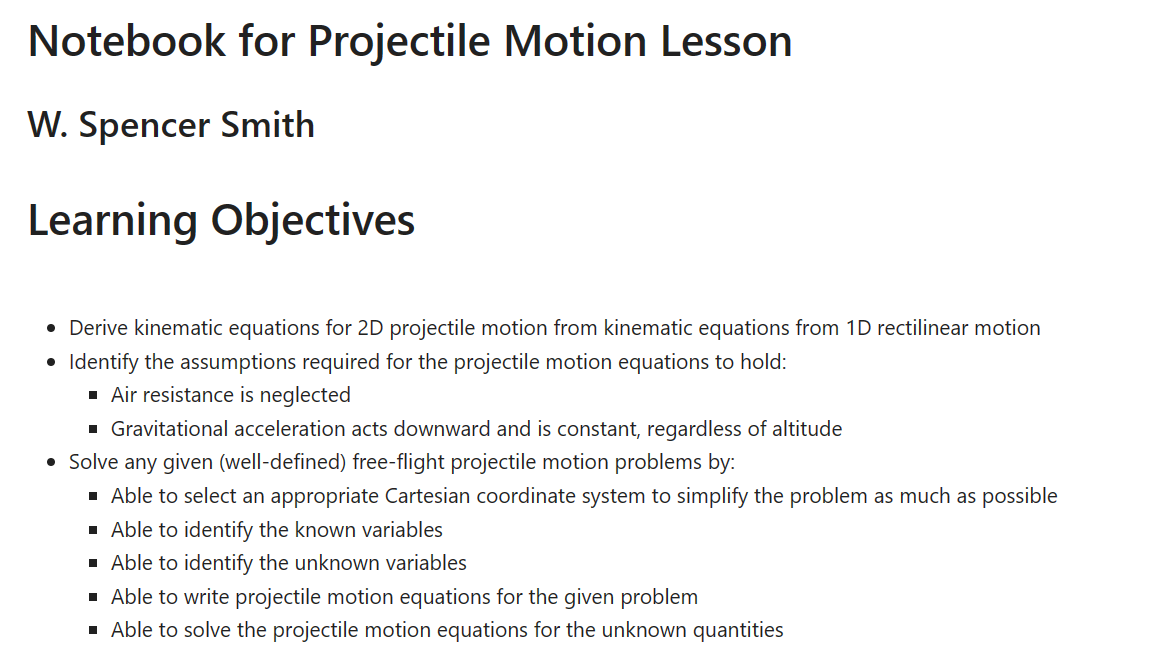
\includegraphics[width=1\textwidth]{figures/learnObj.png}
	\label{fig:learnObj}
\end{figure}

\begin{figure}[h!]
	\caption{Case Problem Generated using Drasil}
	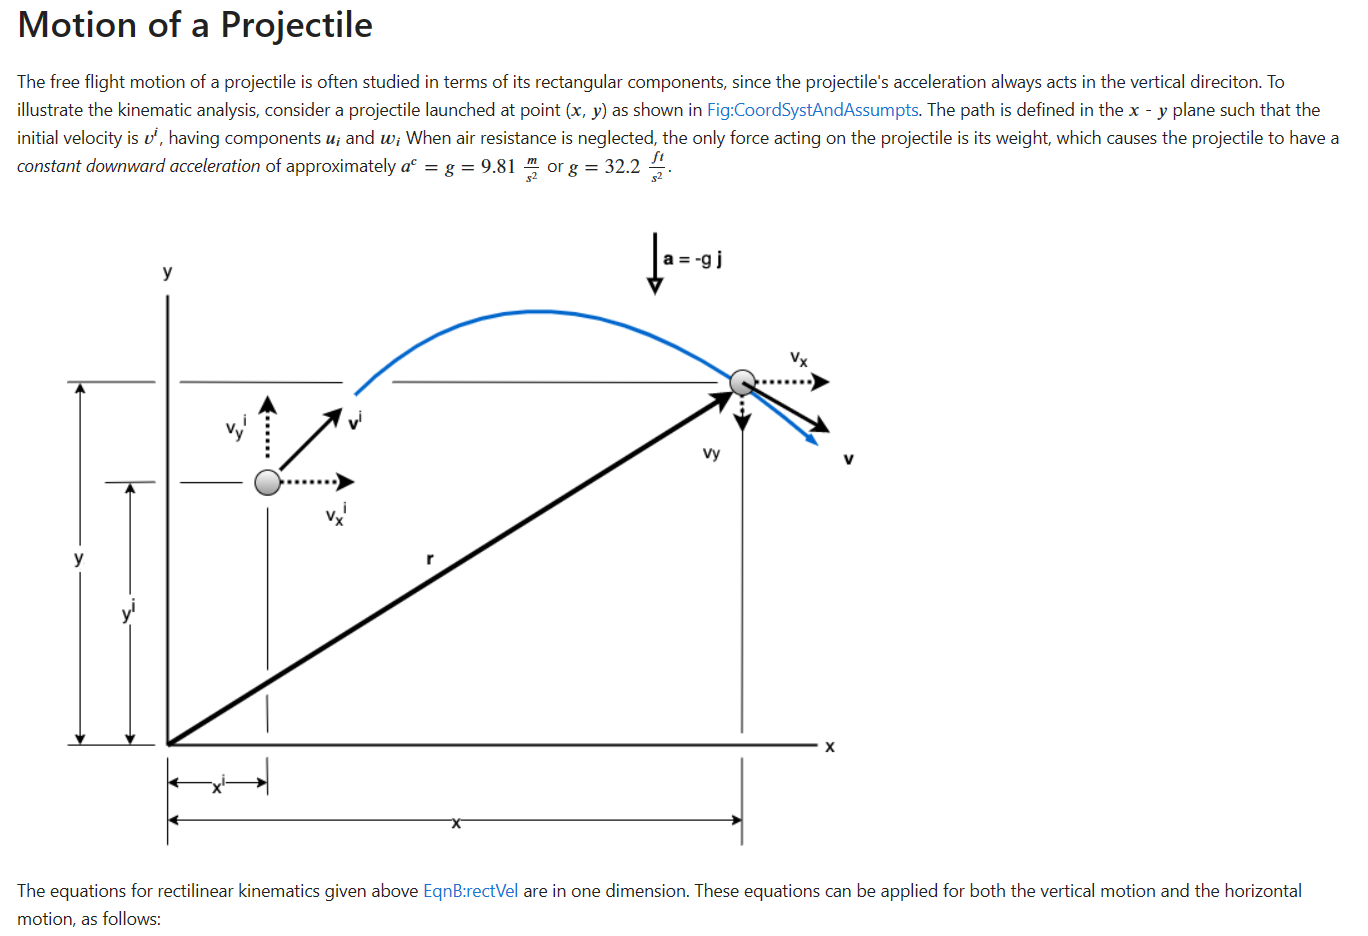
\includegraphics[width=1\textwidth]{figures/caseProb-1.png}
	\label{fig:caseProb-1}
\end{figure}

\begin{figure}[h!]
	\caption{Case Problem Generated using Drasil Cont.}
	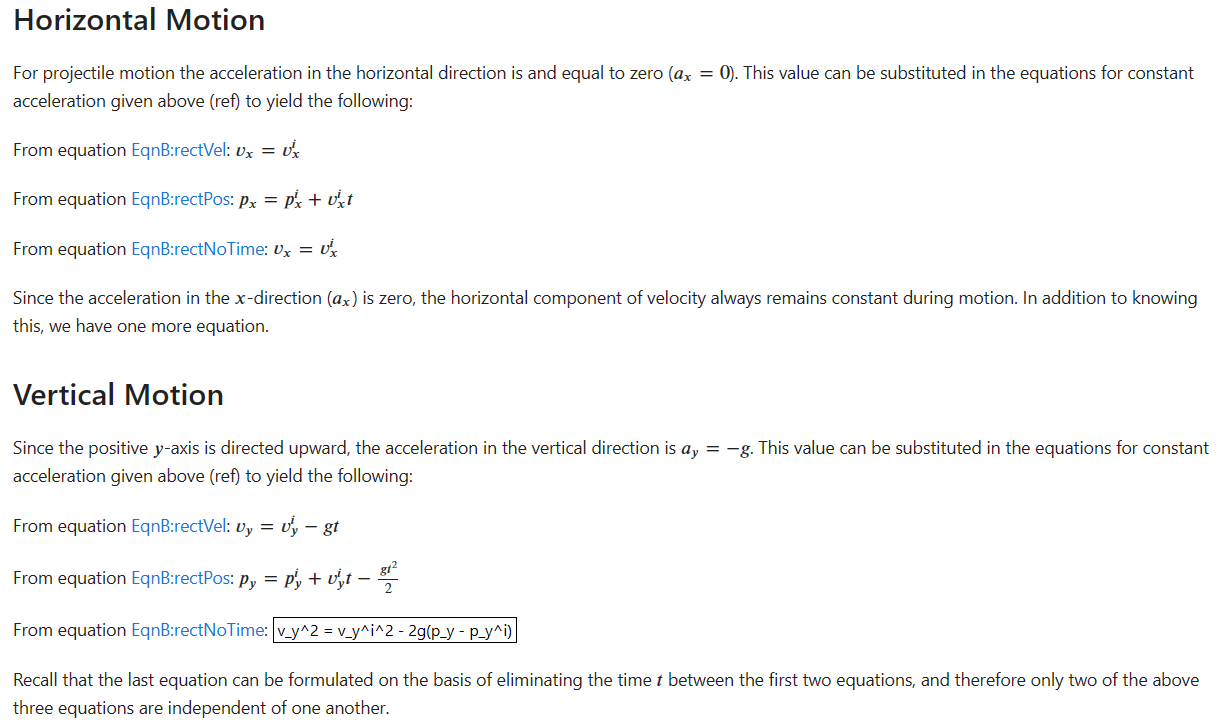
\includegraphics[width=1\textwidth]{figures/caseProb-2.png}
	\label{fig:caseProb-2}
\end{figure}

\begin{figure}[h!]
	\caption{Case Problem Generated using Drasil Cont.}
	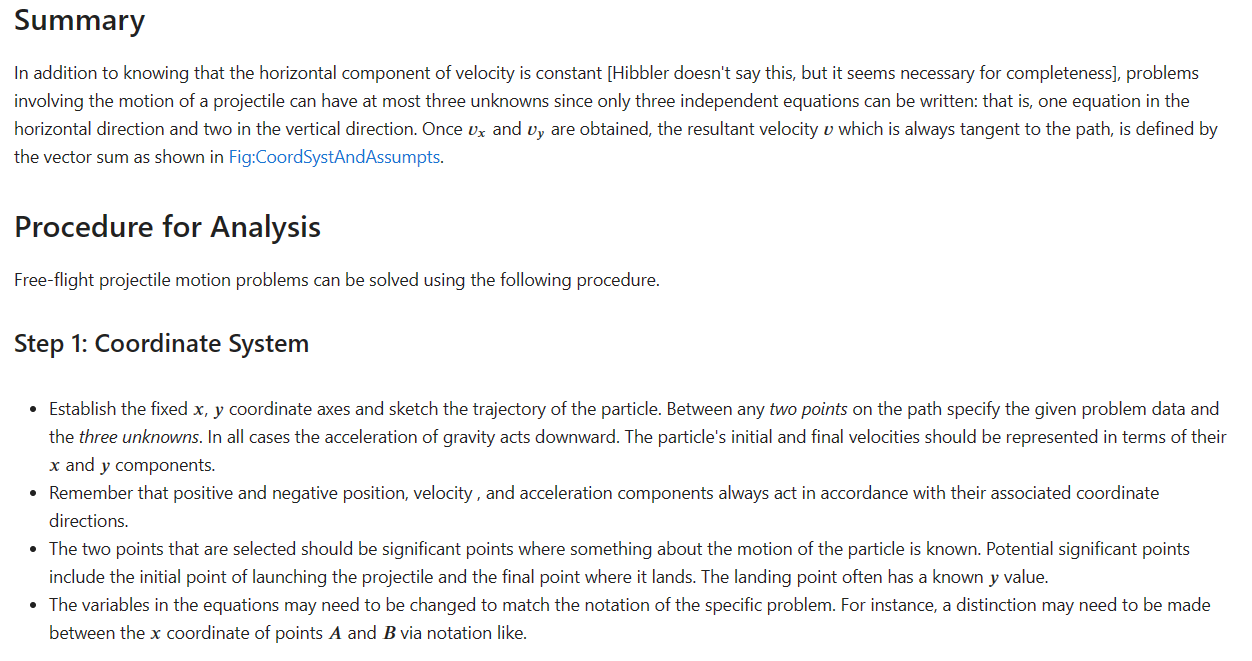
\includegraphics[width=1\textwidth]{figures/caseProb-3.png}
	\label{fig:caseProb-3}
\end{figure}

\begin{figure}[h!]
	\caption{Case Problem Generated using Drasil Cont.}
	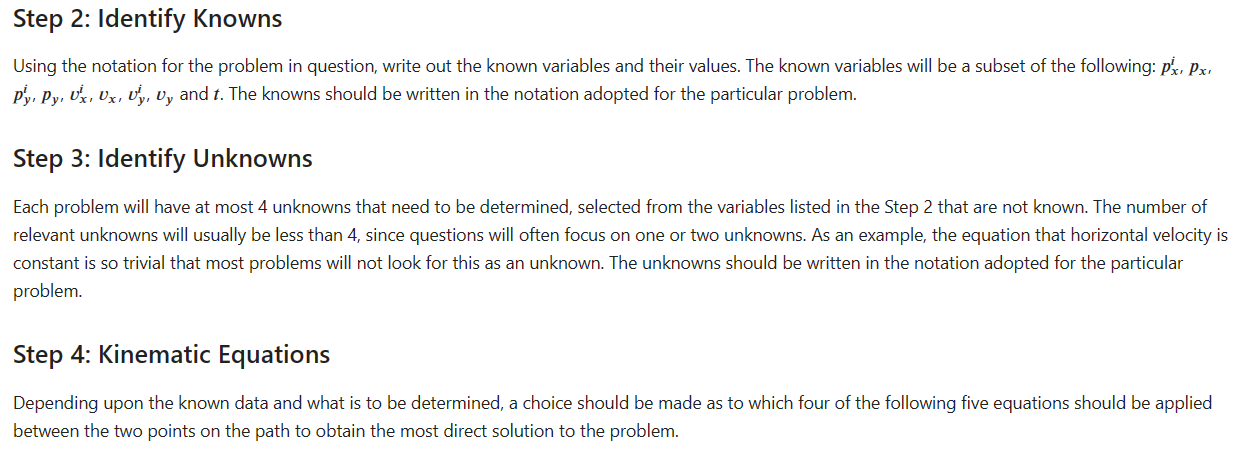
\includegraphics[width=1\textwidth]{figures/caseProb-4.png}
	\label{fig:caseProb-4}
\end{figure}

\begin{figure}[h!]
	\caption{Case Problem Generated using Drasil Cont.}
	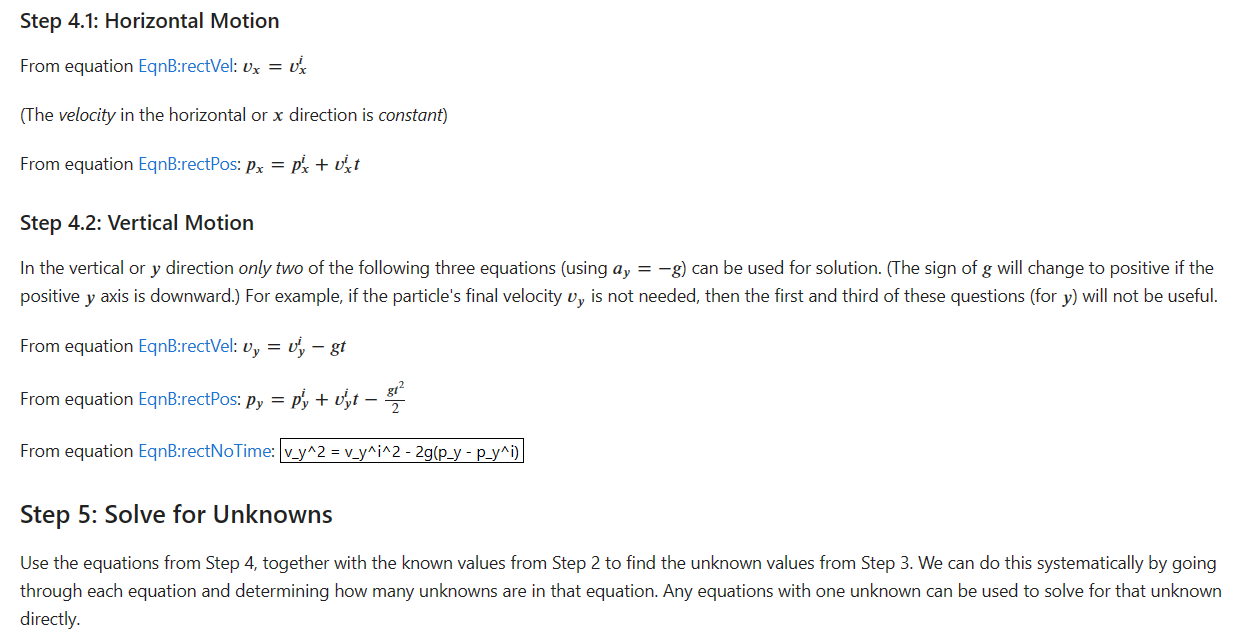
\includegraphics[width=1\textwidth]{figures/caseProb-5.png}
	\label{fig:caseProb-5}
\end{figure}


